\documentclass[conference]{IEEEtran}
\usepackage{cite}
\usepackage{amsmath,amssymb,amsfonts}
\usepackage{graphicx}
\usepackage{booktabs}
\graphicspath{{figs_extracted/}}

\title{Region-Aware ResNet-18 with Learnable Anatomical Embeddings for Facial Acne Severity Classification}

\begin{document}
\maketitle

\begin{abstract}
Acne vulgaris is one of the most prevalent dermatological conditions worldwide, making continuous assessment of its severity a significant challenge for teledermatology applications. Automated acne severity assessment represents a promising application of artificial intelligence to support remote patient monitoring. However, many existing approaches rely on computationally expensive architectures or multi-stage lesion detection, which often limits practical deployment. This work proposes a region-aware framework in which five facial anatomical regions are automatically extracted using a custom YOLOv8 detector and classified by a lightweight, region-aware ResNet-18 network that incorporates learnable anatomical embeddings. The model was evaluated on the public ACNE04 and Acne Level datasets for four-level acne severity classification, including analyses of regional performance, robustness, and prediction confidence. The proposed approach achieved 95.0\% accuracy and a weighted F1-score of 0.95, maintaining consistent performance across facial regions and stable behavior under slight input variations. These results indicate that the proposed framework offers an effective balance between predictive performance, computational efficiency, and practical applicability for AI-assisted acne severity assessment.
\end{abstract}

\begin{IEEEkeywords}
Acne vulgaris, acne severity classification, deep learning, ResNet-18, anatomical embeddings, teledermatology.
\end{IEEEkeywords}

\section{Introduction}
Acne vulgaris is one of the most prevalent inflammatory skin diseases worldwide, affecting approximately 85\% of adolescents and young adults. Beyond dermatological manifestations, moderate to severe acne can lead to permanent scarring and significant psychosocial consequences, including anxiety, depression, and reduced self-esteem. Given that treatment efficacy depends on continuous assessment of disease severity, frequent clinical monitoring is essential~\cite{vasam2023,yli2024}.

The growing advancements in teledermatology have expanded access to dermatological care by enabling remote assessment of skin conditions via images captured with mobile devices~\cite{lenuta2025,heng2020}. Concurrently, recent advances in artificial intelligence and deep learning have significantly enhanced automated analysis of dermatological images, with convolutional neural networks achieving promising results in lesion detection, segmentation, and disease classification~\cite{layton2025,samuels2020}.

Despite advancements, automated assessment of acne severity remains challenging. Most existing approaches rely on multi-stage pipelines in which individual lesions are first detected and subsequently quantified to estimate disease severity~\cite{layton2021,morshed2023,tasneem2023}. Although effective, these strategies increase computational complexity, require lesion-level annotations, propagate errors across stages, and are less suitable for resource-constrained environments. Furthermore, most studies evaluate performance primarily through global classification metrics, with limited investigation into regional consistency, robustness, and prediction confidence---aspects essential for reliable AI-assisted clinical decision support~\cite{eichenfield2021,wongvibulsin2024,reynolds2024}.

To overcome these limitations, this work proposes a region-aware framework for classifying facial acne severity. The framework combines automatic extraction of facial anatomical regions using a custom YOLOv8 detector with a lightweight, region-aware ResNet-18 network that incorporates learnable anatomical embeddings. This design explicitly integrates anatomical context while maintaining a single shared convolutional backbone, thereby reducing computational complexity.

The main contributions are:
\begin{itemize}
\item A region-aware framework combining YOLOv8-based anatomical extraction with a lightweight ResNet-18 using learnable embeddings.
\item A comprehensive experimental evaluation on merged ACNE04 and Acne Level datasets, including global, regional, robustness, and confidence analyses.
\item An extended evaluation protocol oriented to operational deployment in teledermatology scenarios.
\end{itemize}

The remainder of this paper is organized as follows. Section~II reviews recent studies on AI-based acne severity assessment. Section~III describes the proposed architecture, datasets, and experimental protocol. Section~IV presents experimental results and discussion. Section~V concludes the paper and outlines future research directions.

\section{Related Work}
\subsection{Automatic Acne Severity Assessment}
Recent advances in deep learning have improved automated assessment of acne severity from facial images. Existing approaches can be categorized into lesion-based multi-stage pipelines and direct severity classification models~\cite{choy2023,huynh2022,lin2022,liu2022}.

Multi-stage approaches first detect individual acne lesions and then assess severity based on lesion count, type, or distribution. Architectures based on Faster R-CNN, YOLO, and hybrid detection-and-classification frameworks have demonstrated competitive performance~\cite{huynh2022,wen2022,lin2023}. However, these approaches rely on detailed lesion-level annotations, entail higher computational costs, and make classification sensitive to detection failures~\cite{wongvibulsin2024,reynolds2024}.

Direct classification models estimate acne severity from facial images without explicit lesion detection. CNN-based architectures---including ResNet, EfficientNet, and hybrid CNN-transformer models---have shown promising results while simplifying inference~\cite{lin2022,lin2023,gao2025}. Transformer-based models generally require greater computational resources, whereas lightweight CNNs such as ResNet-18 offer a favorable balance between predictive performance and efficiency.

\subsection{Research Gap}
Despite recent progress, significant challenges remain for widespread use of automated acne severity classification in teledermatology. Many solutions achieve good experimental performance but rely on complex multi-stage architectures, increasing computational cost and hindering deployment. Several approaches also require detailed lesion annotations, limiting scalability~\cite{huynh2022,nguyen2024,gazeau2024}.

Another important aspect is evaluation design. Most studies focus on traditional performance metrics, while robustness, prediction stability, performance across facial regions, and model confidence receive comparatively little attention~\cite{choy2023}. In clinical applications, understanding reliability is as important as average accuracy, especially when the system serves as decision support.

In contrast, this paper uses a custom YOLOv8 detector~\cite{sapkota2025} exclusively during preprocessing to locate five facial regions. Severity classification is then performed by a single region-aware ResNet-18 with learnable embeddings. This strategy preserves anatomical context without lesion-level annotations, multiple specialized models, or computationally expensive attention mechanisms. The evaluation extends conventional analysis with regional consistency, robustness, and confidence assessment.

\section{Materials and Methods}
The proposed framework performs automatic classification of facial acne severity by combining anatomical information from the face. Instead of analyzing the face as a single image, the method identifies key anatomical regions and incorporates this information through learnable embeddings. Figure~\ref{fig:pipeline} summarizes the complete pipeline.

\begin{figure}[!t]
\centering
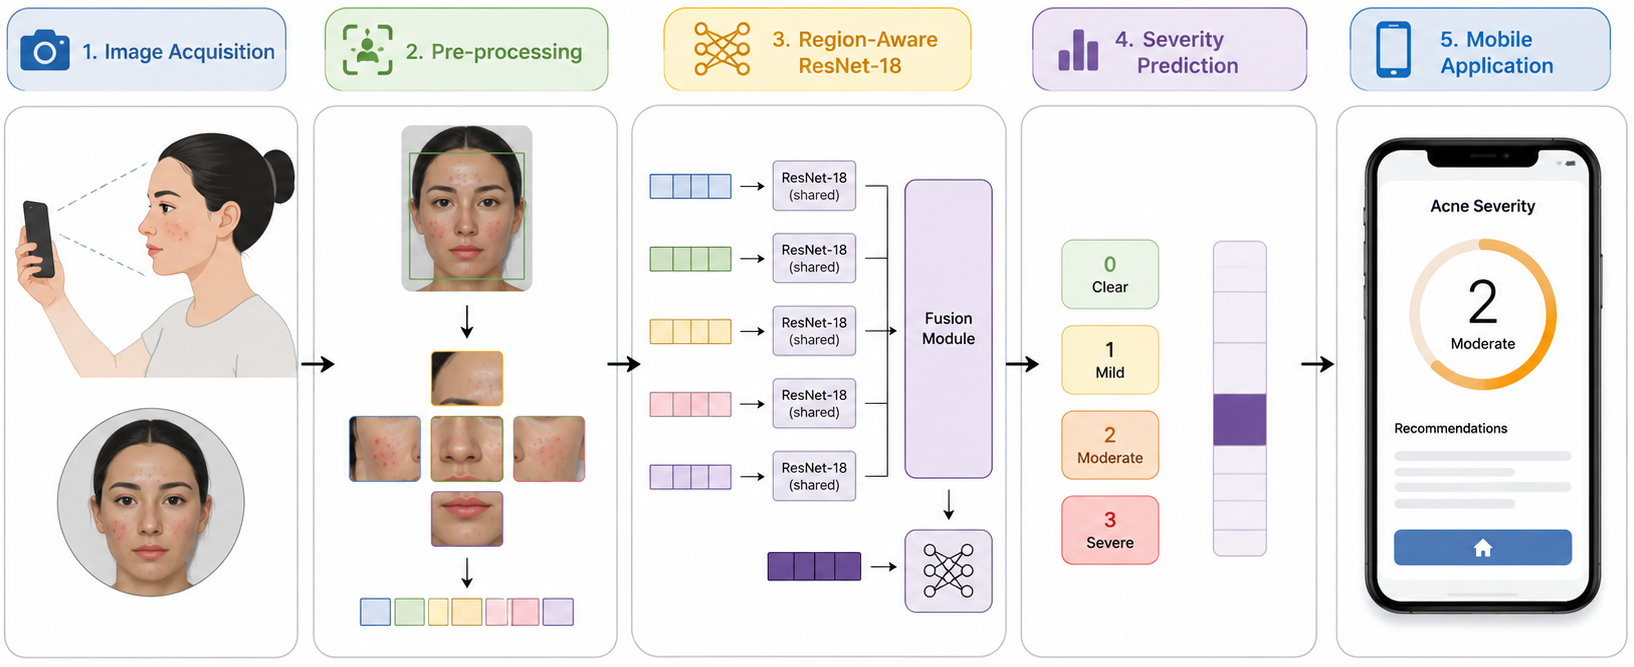
\includegraphics[width=\linewidth]{img_p3_0.png}
\caption{Overview of the proposed region-aware acne severity assessment pipeline.}
\label{fig:pipeline}
\end{figure}

Facial images are pre-processed and divided into anatomical regions. Each region is analyzed by the proposed ResNet-18 architecture, which combines visual features with learnable embeddings to estimate acne severity.

\subsection{Datasets and Pre-processing}
The framework was evaluated using ACNE04~\cite{hettich2019} and Acne Level~\cite{saiman2021}, both following Hayashi's four-level severity scale~\cite{reynolds2024}. The datasets were combined to increase diversity and assess generalization under different acquisition conditions. The merged corpus was randomly split into training (70\%), validation (15\%), and test (15\%) subsets. Table~\ref{tab:datasets} summarizes dataset characteristics.

\begin{table}[!t]
\caption{Characteristics of the datasets used in this study.}
\label{tab:datasets}
\centering
\begin{tabular}{lcc}
\toprule
Characteristic & ACNE04 & Acne Level \\
\midrule
Images & 1,406 & 1,457 \\
Classes & 4 & 4 \\
Severity scale & Hayashi (0--3) & Hayashi (0--3) \\
Experimental use & Merged (70/15/15) & Merged (70/15/15) \\
\bottomrule
\end{tabular}
\end{table}

A custom YOLOv8 detector localized forehead, left cheek, right cheek, nose, and chin (Fig.~\ref{fig:regions}). Each extracted region was resized to $224\times224$ pixels and normalized. The merged dataset partition was performed before training to ensure independent evaluation.

\begin{figure}[!t]
\centering
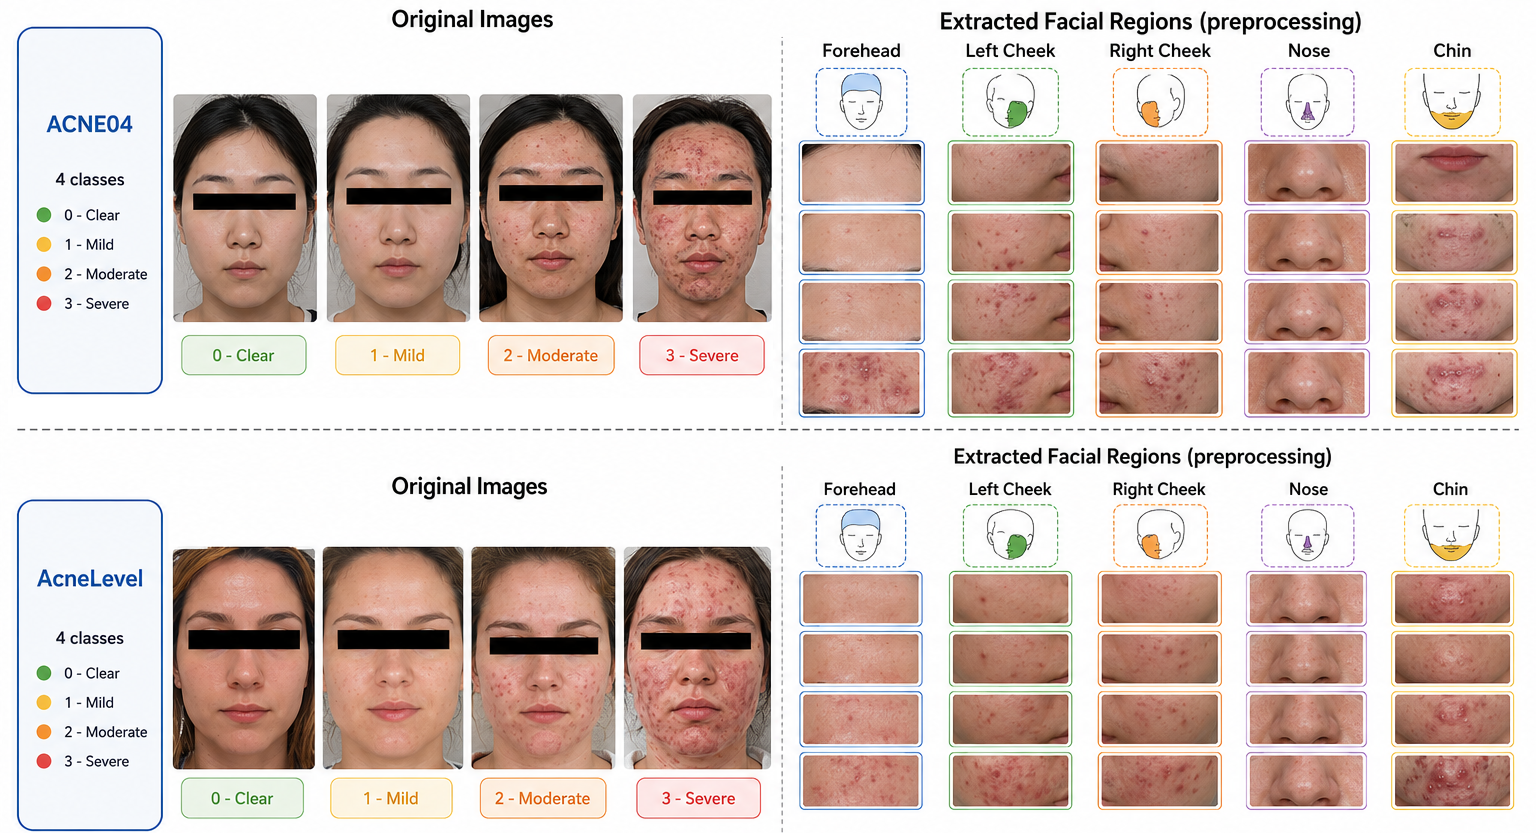
\includegraphics[width=\linewidth]{img_p3_1.png}
\caption{Dataset samples and five automatically extracted facial anatomical regions.}
\label{fig:regions}
\end{figure}

\subsection{Proposed Region-Aware ResNet-18}
After preprocessing, each anatomical facial region is processed independently. The model receives a cropped facial region and its anatomical index, used to retrieve the corresponding learnable embedding (Fig.~\ref{fig:arch}).

\begin{figure}[!t]
\centering
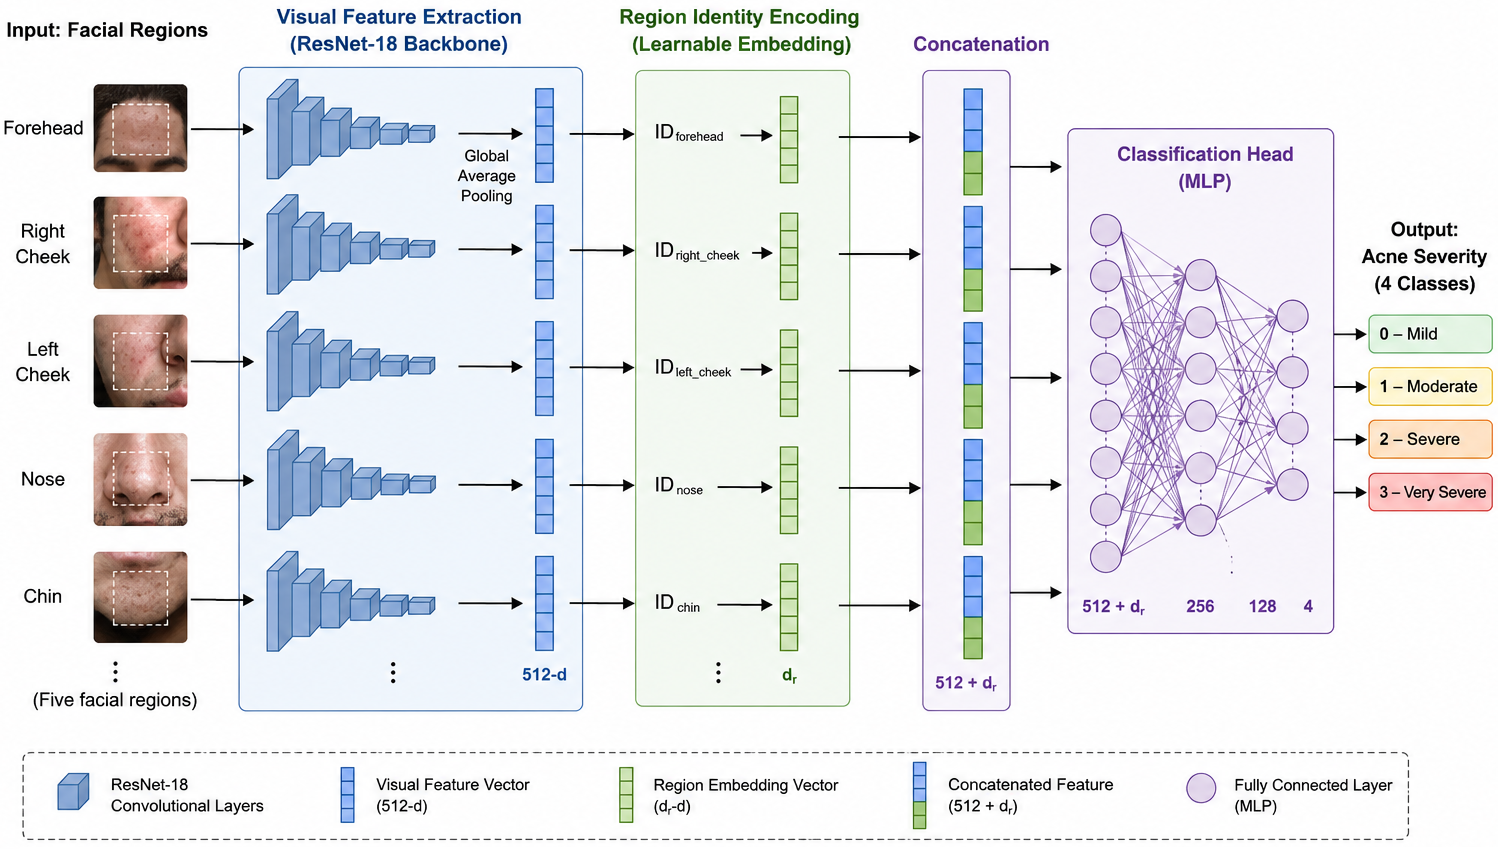
\includegraphics[width=\linewidth]{img_p3_2.png}
\caption{Proposed region-aware ResNet-18 architecture.}
\label{fig:arch}
\end{figure}

Let $x_r$ denote the cropped image of region $r$, where $r\in\{1,\ldots,5\}$. Visual features are extracted by a ResNet-18 backbone $\phi(\cdot)$:
\begin{equation}
f_r = \phi(x_r),
\end{equation}
where $f_r\in\mathbb{R}^{512}$. Each region is associated with a learnable embedding matrix $E\in\mathbb{R}^{5\times64}$:
\begin{equation}
e_r = E[r],
\end{equation}
where $e_r\in\mathbb{R}^{64}$. Visual and anatomical representations are concatenated:
\begin{equation}
z_r = f_r \oplus e_r,
\end{equation}
with $z_r\in\mathbb{R}^{576}$. The fused representation is processed by a classification head with fully connected layers, batch normalization, ReLU, and dropout to produce logits $o_r=g(z_r)$ for four severity classes. Class probabilities are obtained with
\begin{equation}
p_{r,c}=\frac{\exp(o_{r,c})}{\sum_{k=1}^{C}\exp(o_{r,k})},
\end{equation}
and the predicted severity is $\hat{y}_r=\arg\max_c p_{r,c}$.

Unlike conventional ResNet-18, the proposed architecture incorporates anatomical identity through learnable embeddings while maintaining a single shared backbone for all facial regions. Consequently, the approach learns region-specific visual patterns with only a slight increase in trainable parameters, preserving computational efficiency.

\subsection{Training Strategy}
Training was conducted in a supervised multi-class scenario using weighted cross-entropy to mitigate class imbalance. The Adam optimizer was used with batch size 16 and 40 epochs. Data augmentation included horizontal flipping, rotation, color jittering, Gaussian blurring, and random erasing. Learning rate was adjusted with ReduceLROnPlateau, and early stopping preserved the best model. Implementation used PyTorch~\cite{paszke2019} on an NVIDIA RTX 3060 GPU. Main hyperparameters are listed in Table~\ref{tab:hyper}.

\begin{table}[!t]
\caption{Main hyperparameters used during training.}
\label{tab:hyper}
\centering
\begin{tabular}{ll}
\toprule
Parameter & Value \\
\midrule
Framework & PyTorch \\
Backbone & ResNet-18 \\
Optimizer & Adam \\
Loss function & Weighted cross-entropy \\
Learning rate & 0.0001 \\
Scheduler & ReduceLROnPlateau \\
Batch size & 16 \\
Maximum epochs & 40 \\
Data augmentation & Flip, rotation ($\pm25^\circ$), color jitter \\
Regularization & Batch normalization and dropout \\
Hardware & NVIDIA GeForce RTX 3060 (12 GB) \\
\bottomrule
\end{tabular}
\end{table}

These training strategies were selected to improve robustness while maintaining a lightweight architecture suitable for practical implementation. Combined with anatomical embeddings, they contributed to stable convergence and consistent performance across facial regions evaluated in this study.

\subsection{Experimental Protocol}
The framework was evaluated using accuracy, precision, recall, and weighted F1-score:
\begin{align}
\mathrm{Accuracy} &= \frac{TP+TN}{TP+TN+FP+FN}, \\
\mathrm{Precision} &= \frac{TP}{TP+FP}, \quad
\mathrm{Recall} = \frac{TP}{TP+FN}, \\
\mathrm{F1} &= \frac{2\cdot \mathrm{Precision}\cdot \mathrm{Recall}}{\mathrm{Precision}+\mathrm{Recall}},
\end{align}
where $TP$, $TN$, $FP$, and $FN$ denote true positives, true negatives, false positives, and false negatives, respectively. Precision, recall, and F1-score were computed per class and aggregated with weighted averaging.

In addition, three complementary perspectives were considered: overall classification performance, consistency across anatomical regions, and operational robustness through repeated perturbation experiments and confidence analysis. Together, these analyses characterize predictive performance, regional consistency, stability, and reliability for AI-assisted teledermatology.

\section{Experimental Results}
The experimental evaluation investigates the proposed framework from multiple perspectives. In addition to conventional classification metrics, we examined performance across anatomical regions, stability during repeated evaluations, and confidence associated with model decisions. Together, these analyses provide a comprehensive understanding of model behavior under conditions relevant to teledermatology.

\subsection{Overall Classification Performance}
The held-out test set contains 1,090 images. Table~\ref{tab:overall} summarizes per-class results obtained with the unified workflow described in Section~III. The framework achieved 95.0\% accuracy and weighted F1-score of 0.95, demonstrating reliable discrimination among four facial acne severity levels. Mild and very severe classes were classified with higher precision, whereas severe yielded the lowest F1-score (0.90), as expected for adjacent-grade ambiguity.

\begin{table}[!t]
\caption{Overall classification performance of the proposed architecture.}
\label{tab:overall}
\centering
\begin{tabular}{lcccc}
\toprule
Class & Prec. & Rec. & F1 & Support \\
\midrule
Mild & 0.96 & 0.95 & 0.95 & 318 \\
Moderate & 0.94 & 0.94 & 0.94 & 412 \\
Severe & 0.88 & 0.92 & 0.90 & 110 \\
Very severe & 1.00 & 1.00 & 1.00 & 250 \\
\midrule
Weighted avg. & 0.95 & 0.95 & 0.95 & 1090 \\
\midrule
Overall accuracy & \multicolumn{4}{c}{95.0\%} \\
\bottomrule
\end{tabular}
\end{table}

The confusion matrix in Fig.~\ref{fig:conf} shows that most misclassifications occurred between moderate and severe classes, while confusion between mild and very severe was negligible. This indicates that errors are concentrated in clinically adjacent categories.

\begin{figure}[!t]
\centering
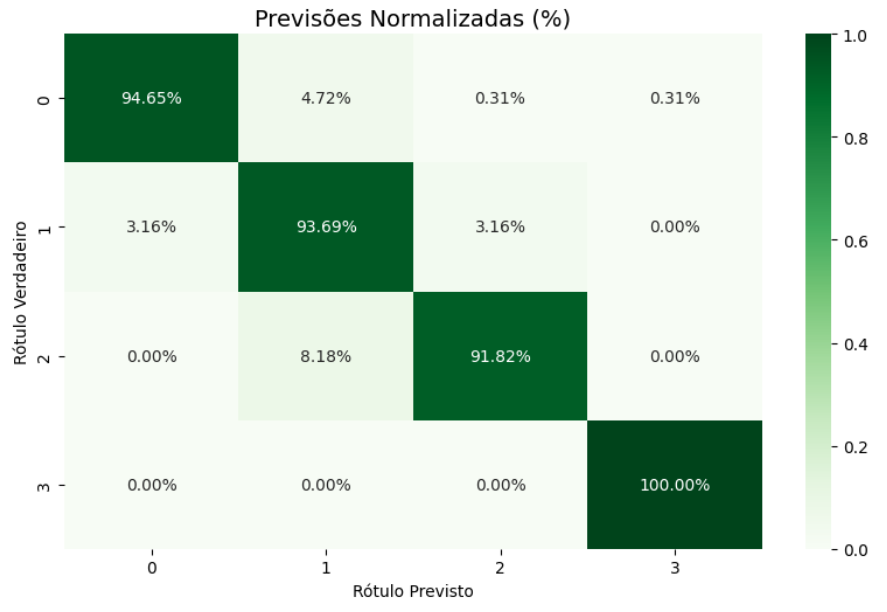
\includegraphics[width=\linewidth]{img_p5_0.png}
\caption{Row-normalized confusion matrix (\%) obtained on the test set.}
\label{fig:conf}
\end{figure}

\subsection{Regional Performance Analysis}
Classification performance was analyzed independently for each facial region (Table~\ref{tab:regions}). Weighted F1 ranged from 0.93 to 0.99. Forehead achieved the highest score (0.99), while chin and left cheek were comparatively harder (0.93), likely due to texture variability, facial hair, shadows, and illumination effects. Even in these regions, performance remained consistently high.

\begin{table}[!t]
\caption{Weighted classification performance according to facial region.}
\label{tab:regions}
\centering
\begin{tabular}{lcccc}
\toprule
Region & Prec. & Rec. & F1 & Support \\
\midrule
Forehead & 0.99 & 0.99 & 0.99 & 93 \\
Chin & 0.94 & 0.93 & 0.93 & 329 \\
Nose & 0.97 & 0.97 & 0.97 & 103 \\
Left cheek & 0.94 & 0.93 & 0.93 & 169 \\
Right cheek & 0.96 & 0.96 & 0.96 & 396 \\
\bottomrule
\end{tabular}
\end{table}

These results indicate that anatomical embeddings capture region-specific contextual information while allowing all facial regions to be processed by a single shared network.

\subsection{Robustness and Confidence Analysis}
High classification accuracy alone is not sufficient for clinical applications. In teledermatology, images may be acquired under different lighting conditions, camera positions, and smartphone devices, making it essential to verify whether the framework maintains stable performance under small input variations.

To assess this aspect, 30 independent robustness experiments were performed with small random perturbations. Figure~\ref{fig:stability} shows the resulting accuracy distribution. Mean accuracy was 94.41\% with standard deviation of 0.46, indicating stable behavior across repeated evaluations and resilience to variations commonly encountered during smartphone image acquisition.

Confidence analysis using maximum softmax probability showed that most correct predictions received scores close to 1.0, while a smaller subset of incorrect predictions also received high confidence, revealing occasional overconfidence in visually challenging cases. These findings complement global and regional analyses and support future uncertainty-aware triage strategies for clinical decision support.

\begin{figure}[!t]
\centering
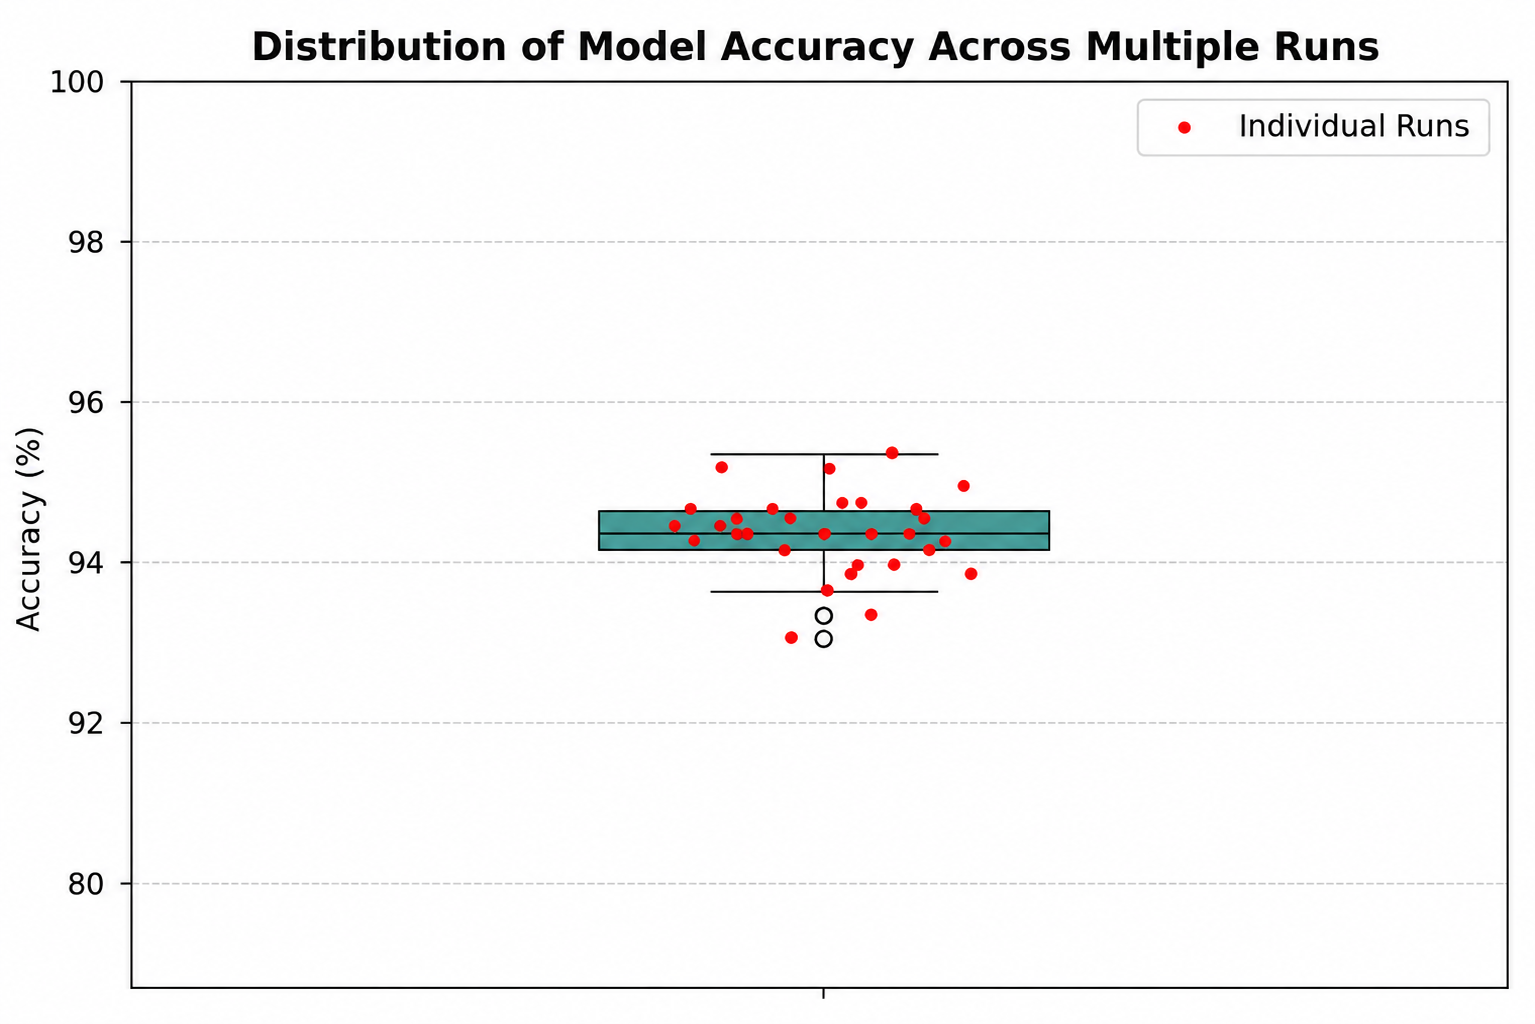
\includegraphics[width=0.92\linewidth]{img_p6_0.png}
\caption{Accuracy distribution obtained from 30 independent robustness experiments.}
\label{fig:stability}
\end{figure}

\section{Discussion}
Experimental results demonstrate that incorporating anatomical information enables a lightweight convolutional architecture to achieve high predictive performance while maintaining computational efficiency. Unlike multi-specialized or computationally intensive approaches, the proposed framework enriches visual representation with anatomical context while retaining a single shared ResNet-18 backbone.

Regional analysis demonstrated consistent performance across all facial regions, including challenging areas such as cheeks and chin. Low variability during robustness testing indicates resilience to acquisition variations commonly encountered in teledermatology. Although some high-confidence misclassifications were identified, the proposed system should serve as clinical decision support rather than a substitute for expert assessment.

Beyond facial acne severity classification, the proposed approach represents a general strategy for incorporating anatomical context into lightweight CNNs and may benefit other biomedical image analysis tasks where anatomical location plays a significant role in clinical decision-making.

\section{Limitations}
The experimental evaluation was conducted using two publicly available datasets that do not fully represent patient diversity, imaging devices, and acquisition conditions encountered in everyday clinical practice. Evaluating the approach on independent datasets and more heterogeneous populations remains an important next step.

Another limitation concerns confidence estimates from the softmax classifier. Although most predictions were consistent with observed performance, a small number of incorrect predictions also received high confidence scores. Probability calibration and uncertainty estimation techniques could further enhance reliability. These limitations do not diminish the main contribution of this work; instead, they indicate next steps for transforming the framework into a robust, clinically validated teledermatology tool.

\section{Conclusion}
This study presented a region-aware ResNet-18 architecture for automatic classification of facial acne severity, explicitly incorporating learnable anatomical region embeddings into a lightweight convolutional neural network. Unlike conventional lesion-based workflows or computationally intensive deep learning models, the proposed framework integrates anatomical context into a single shared backbone, offering an efficient solution for teledermatology-oriented analysis.

Experimental results demonstrated high predictive performance with consistent behavior across facial regions and stability during repeated assessments. Beyond conventional metrics, the evaluation incorporated regional consistency, robustness, and predictive confidence analyses, providing a broader characterization of model behavior. Future work includes external validation using larger and more diverse populations, probability calibration, explainable AI techniques, and prospective clinical evaluation of teledermatology systems. Overall, the proposed framework represents a practical and efficient solution for AI-assisted facial acne severity assessment, with significant potential for remote clinical decision support.



\begin{thebibliography}{99}
\bibitem{vasam2023}M. Vasam, A. Korivi, and K. M. Balli, ``Acne vulgaris: A review of the pathophysiology, treatment, and recent nanotechnology-based advances,'' \emph{Biomedicines}, vol. 11, no. 12, Art. no. 3284, 2023.
\bibitem{yli2024}Y. Li, X. Hu, G. Dong, X. Wang, and T. Liu, ``Acne treatment: research progress and new perspectives,'' \emph{Frontiers in Medicine}, vol. 11, Art. no. 1366957, 2024.
\bibitem{lenuta2025}G. D. Lenut\`{a} \emph{et al.}, ``The epidemiology of acne in the current era: trends and clinical implications,'' \emph{Cosmetics}, vol. 12, no. 3, 2025.
\bibitem{heng2020}A. H. Heng and F. T. Chew, ``Systematic review of the epidemiology of acne vulgaris,'' \emph{Scientific Reports}, vol. 10, Art. no. 5754, 2020.
\bibitem{layton2025}A. M. Layton, ``The burden of acne vulgaris on health-related quality of life,'' \emph{Dermatology and Therapy}, vol. 15, 2025.
\bibitem{samuels2020}D. V. Samuels \emph{et al.}, ``Acne vulgaris and risk of depression and anxiety: A meta-analytic review,'' \emph{J. Amer. Acad. Dermatol.}, vol. 83, no. 2, pp. 532--541, 2020.
\bibitem{layton2021}A. M. Layton, D. Thiboutot, and J. Tan, ``Reviewing the global burden of acne: how could we improve care to reduce the burden?'' \emph{Brit. J. Dermatol.}, vol. 184, no. 2, pp. 219--225, 2021.
\bibitem{morshed2023}A. S. Morshed \emph{et al.}, ``Understanding the impact of acne vulgaris and associated psychological distress on self-esteem and quality of life,'' \emph{Scientific Reports}, vol. 13, Art. no. 15841, 2023.
\bibitem{tasneem2023}T. Tasneem \emph{et al.}, ``Effects of acne severity and acne-related quality of life on depressive symptoms among adolescents and young adults,'' \emph{Frontiers in Psychology}, vol. 14, Art. no. 1213540, 2023.
\bibitem{eichenfield2021}D. Z. Eichenfield, J. Sprague, and L. F. Eichenfield, ``Management of acne vulgaris: a review,'' \emph{JAMA}, vol. 326, no. 20, pp. 2055--2067, 2021.
\bibitem{wongvibulsin2024}S. Wongvibulsin \emph{et al.}, ``Current state of dermatology mobile applications with artificial intelligence features,'' \emph{JAMA Dermatology}, vol. 160, no. 6, pp. 617--626, 2024.
\bibitem{reynolds2024}R. V. Reynolds \emph{et al.}, ``Guidelines of care for the management of acne vulgaris,'' \emph{J. Amer. Acad. Dermatol.}, vol. 90, no. 5, pp. 1006--1032, 2024.
\bibitem{choy2023}S. P. Choy \emph{et al.}, ``Systematic review of deep learning image analyses for the diagnosis and monitoring of skin disease,'' \emph{npj Digital Medicine}, vol. 6, no. 1, Art. no. 180, 2023.
\bibitem{huynh2022}Q. T. Huynh \emph{et al.}, ``Automatic acne object detection and acne severity grading using smartphone images and artificial intelligence,'' \emph{Diagnostics}, vol. 12, no. 8, Art. no. 1879, 2022.
\bibitem{lin2022}Y. Lin \emph{et al.}, ``KIEGLFN: A unified acne grading framework on face images,'' \emph{Computer Methods and Programs in Biomedicine}, vol. 221, Art. no. 106911, 2022.
\bibitem{liu2022}S. Liu \emph{et al.}, ``AcneGrader: An ensemble pruning of the deep learning base models to grade acne,'' \emph{Skin Research and Technology}, vol. 28, no. 5, pp. 677--688, 2022.
\bibitem{wen2022}H. Wen \emph{et al.}, ``Acne detection and severity evaluation with interpretable convolutional neural network models,'' \emph{Technology and Health Care}, vol. 30, no. 1, pp. 143--153, 2022.
\bibitem{lin2023}Y. Lin \emph{et al.}, ``DED: Diagnostic evidence distillation for acne severity grading on face images,'' \emph{Expert Systems with Applications}, vol. 228, Art. no. 120312, 2023.
\bibitem{nguyen2024}P. K. Nguyen \emph{et al.}, ``ACNE8M: An acnes detection and differential diagnosis system using AI technologies,'' \emph{VNUHCM J. Sci. Technol. Dev.}, vol. 27, no. 3, pp. 3550--3561, 2024.
\bibitem{gazeau2024}L. Gazeau \emph{et al.}, ``AcneAI: A new acne severity assessment method using digital images and deep learning,'' in \emph{Proc. MICCAI}, 2024, pp. 68--78.
\bibitem{gao2025}N. Gao \emph{et al.}, ``Evaluation of an acne lesion detection and severity grading model for Chinese population in online and offline healthcare scenarios,'' \emph{Scientific Reports}, vol. 15, Art. no. 1119, 2025.
\bibitem{viana2025}T. A. S. Viana \emph{et al.}, ``ClearFace: Facial acne detection and classification system using YOLOv11 and EfficientNet-B0,'' in \emph{Proc. SIBGRAPI Extended Papers}, 2025.
\bibitem{he2016resnet}K. He, X. Zhang, S. Ren, and J. Sun, ``Deep residual learning for image recognition,'' in \emph{Proc. CVPR}, 2016, pp. 770--778.
\bibitem{paszke2019}A. Paszke \emph{et al.}, ``PyTorch: An imperative style, high-performance deep learning library,'' in \emph{NeurIPS}, vol. 32, 2019.
\bibitem{sapkota2025}R. Sapkota and M. Karkee, ``Ultralytics YOLO evolution: An overview of YOLO26, YOLO11, YOLOv8 and YOLOv5 object detectors for computer vision and pattern recognition,'' arXiv:2510.09653, 2025.
\bibitem{saiman2021}G. Saiman, ``Acne Level dataset,'' May 2021. [Online]. Available: https://www.kaggle.com/datasets/gsaiman/acne-level
\bibitem{hettich2019}M. Hettich, ``ACNE04 dataset,'' Aug. 2019. [Online]. Available: https://www.kaggle.com/datasets/manuelhettich/acne04
\bibitem{flutter2026}Flutter Documentation, ``Flutter documentation,'' 2026. [Online]. Available: https://docs.flutter.dev
\end{thebibliography}

\end{document}
